\documentclass[xcolor=table, 11pt]{beamer}
\usetheme{Warsaw}
\usepackage[utf8]{inputenc}
\usepackage{vietnam}
\usepackage{sansmathaccent}
\usepackage{amsmath}
\usepackage{amsfonts}
\usepackage{amssymb}
\usepackage{graphics} % thư viện để hiển thị ảnh
\usepackage{caption} % thư viện để đặt caption
\usepackage{booktabs} % thư viện để vẽ table
\usepackage{hyperref} % thư viện để link tới các chương
\usepackage{booktabs}
\usepackage{xcolor}
% \usepackage{neuralnetwork}
\usepackage{tikz}
% \usetikzlibrary{positioning}

%\usepackage{tikz} % thư viện vẽ hình
\pdfmapfile{+sansmathaccent.map}
 
% thông tin bìa slide
\author{PVU, Trong Nghia\\
\textit{Instructor: Ha Minh Dung}}
\title{Multilayer Perceptron for Well Performance Optimization}
\institute{Japan Vietnam Petroleum Company}
 
% đánh số cho caption và footline
\setbeamertemplate{caption}[numbered]
\setbeamertemplate{footline}[frame number]
 
% danh sách các lệnh tự định nghĩa
\newcommand{\argmax}{\arg\!\max}
 
\begin{document}
 
\begin{frame}
\titlepage % tạo trang bìa slide
\end{frame}
 
\begin{frame}{Contents}
\tableofcontents % tạo bảng nội dung
\end{frame}

\section{Introduction}
\subsection{Objectives}
\begin{frame}{Introduction}
The objectives:
    \begin{itemize}
        \item Building new model to predict oil rate based on known features (Gaslift, Gas-oil ratio, water cut...)
        \item Automatic optimize well performance,
        \item For study and research purposes.
    \end{itemize}
Well X1: This well was choose randomly with all below constraints:
    \begin{itemize}
        \item Fully structured data
        \item Time series with no lag time
        \item In RangDong oil field.
    \end{itemize}
\end{frame}
\subsection{Methodology}
\begin{frame}{Methodology}
Fully connected Multi-layer Perceptron (MLP):
    \begin{itemize}
        \item One of the AI method
        \item Easy to use
        \item High performance
        \item Suitable for fully structured data
        \item Suitable for time series forecasting.
    \end{itemize} 
Using Root Mean Squared Error and $R^2$ metrics to evaluate the results.
\end{frame}
\begin{frame}{Introduction}
Sample model of Fully connected MLP:
\def\layersep{2.5cm}
\begin{tikzpicture}[shorten >=1pt,->,draw=black!50, node distance=\layersep]
    \tikzstyle{every pin edge}=[<-,shorten <=1pt]
    \tikzstyle{neuron}=[circle,fill=black!25,minimum size=17pt,inner sep=0pt]
    \tikzstyle{input neuron}=[neuron, fill=green!50];
    \tikzstyle{output neuron}=[neuron, fill=red!50];
    \tikzstyle{hidden neuron}=[neuron, fill=blue!50];
    \tikzstyle{annot} = [text width=4em, text centered]

    % Draw the input layer nodes
    \foreach \name / \y in {1,...,4}
    % This is the same as writing \foreach \name / \y in {1/1,2/2,3/3,4/4}
        \node[input neuron, pin=left:Input \#\y] (I-\name) at (0,-\y) {};

    % Draw the hidden layer nodes
    \foreach \name / \y in {1,...,5}
        \path[yshift=0.5cm]
            node[hidden neuron] (H-\name) at (\layersep,-\y cm) {};

    % Draw the output layer node
    \node[output neuron,pin={[pin edge={->}]right:Output}, right of=H-3] (O) {};

    % Connect every node in the input layer with every node in the
    % hidden layer.
    \foreach \source in {1,...,4}
        \foreach \dest in {1,...,5}
            \path (I-\source) edge (H-\dest);

    % Connect every node in the hidden layer with the output layer
    \foreach \source in {1,...,5}
        \path (H-\source) edge (O);

    % Annotate the layers
    \node[annot,above of=H-1, node distance=1cm] (hl) {Hidden layer};
    \node[annot,left of=hl] {Input layer};
    \node[annot,right of=hl] {Output layer};
\end{tikzpicture}
\end{frame}

% ví dụ cho section introduction
\section{Data preparation}
\begin{frame}{First look dataset}
    \begin{table}[h]
    \caption{Well X1}
    \begin{tabular}{@{}ccccccc@{}}
    \toprule
    \textbf{\begin{tabular}[c]{@{}c@{}}WHFP\\ psi\end{tabular}} & \textbf{\begin{tabular}[c]{@{}c@{}}WHFT\\ deg C\end{tabular}} & \textbf{\begin{tabular}[c]{@{}c@{}}WCT\\ \%bbl/bbl\end{tabular}} & \textbf{\begin{tabular}[c]{@{}c@{}}GOR\\ cf/bbl\end{tabular}} & \textbf{\begin{tabular}[c]{@{}c@{}}BHP\\ psi\end{tabular}} & \textbf{\begin{tabular}[c]{@{}c@{}}Qgl\\ Mcf/d\end{tabular}} & \textbf{\begin{tabular}[c]{@{}c@{}}Qo\\ SBT/D\end{tabular}} \\ \midrule
    902.83                                                      & 29.26                                                         & NaN                                                              & 0                                                             & 4786.92                                                    & 0                                                            & 0                                                           \\
    1118.07                                                     & 30.02                                                         & NaN                                                              & 0                                                             & 3638.66                                                    & 0                                                            & 0                                                           \\
    ...                                                         & ...                                                           & ...                                                              & ...                                                           & ...                                                        & ...                                                          & ...                                                         \\
    204.98                                                      & 62.2                                                          & 91.05                                                            & 333                                                           & 2715.62                                                    & 1104                                                         & 153.27                                                      \\
    202.45                                                      & 62.63                                                         & 91.14                                                            & 329                                                           & 2702.48                                                    & 1096                                                         & 152                                                         \\ \bottomrule
    \end{tabular}
    \end{table}
    \begin{itemize}
        \item 1720 samples
        \item Date: from 6/2/2014 - 2/6/2019 (format: m/d/y)
        \item 42 missing values on WCT (NaN values)
    \end{itemize}
\end{frame}

\begin{frame}{First look dataset}
    \begin{figure}
        \centering
        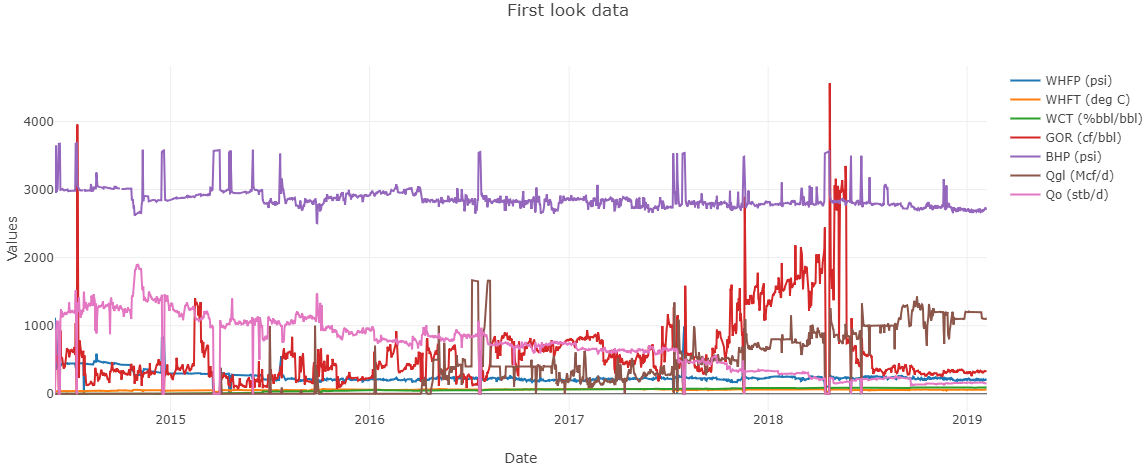
\includegraphics[scale=.38]{fig/first_look.PNG}
        \caption{Original data}
        \label{fig:my_label}
    \end{figure}
\end{frame}

\subsection{Preprocessing}
\begin{frame}{Data cleaning}
Feature selection: Based on dependence of output data on input data.
    \begin{itemize}
        \item Water cut (No outliers detected, so keep it unchange).
        \item Gas oil ratio
        \item Gaslift rate
    \end{itemize}
Output: Oil rate.\\
Cleaning methods:
    \begin{itemize}
        \item Handle outliers (``Mean detection-fill method")
        \item Removing 0 values (in ``gaslift rate" feature)
        \item Handle missing data (Fill with mean value)
    \end{itemize}
\end{frame}

\begin{frame}{Data cleaning}
Mean detection and fill method:
    \begin{itemize}
        \item[Step 1:] From original data, split selected feature into $n$ interval (here $n = 17$)
        \item[Step 2:] In each interval:
            \begin{itemize}
                \item Calculate mean
                \item Compare mean value with all values:\\ 
                if $value < mean - 300$ or $value > mean + 300$ $=>$ fill this value with $mean \pm 30$.
            \end{itemize}
        \item [Step 3:] Loop for all interval.
    \end{itemize}
300 and 30 from analyst's intuition.
\end{frame}
\begin{frame}{Data cleaning}
    \begin{figure}
        \centering
        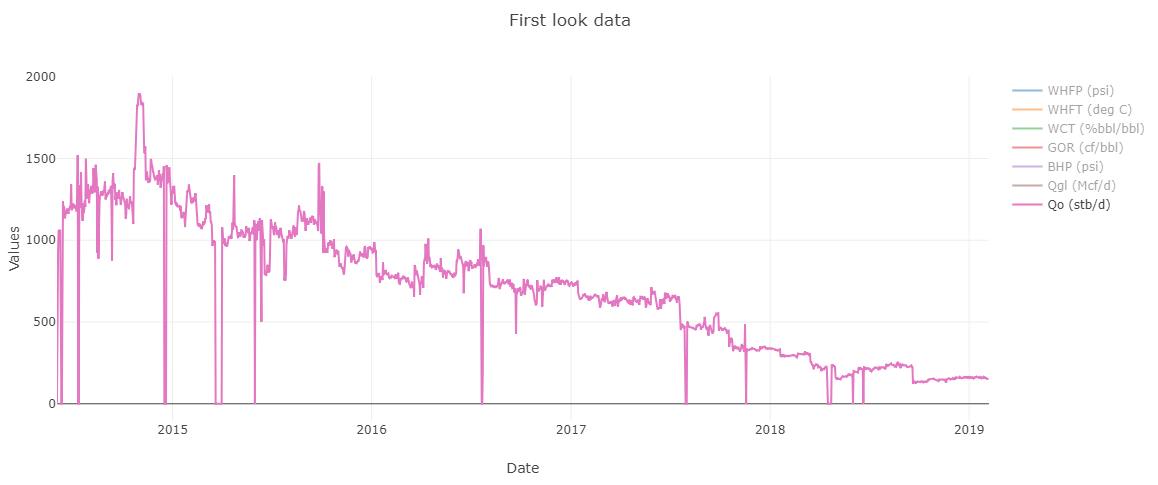
\includegraphics[scale=0.38]{fig/q_oil_before.PNG}
        \caption{Oil rate before remove outliers}
        \label{fig:q_oil_before}
    \end{figure}
\end{frame}
\begin{frame}{Data cleaning}
    \begin{figure}
        \centering
        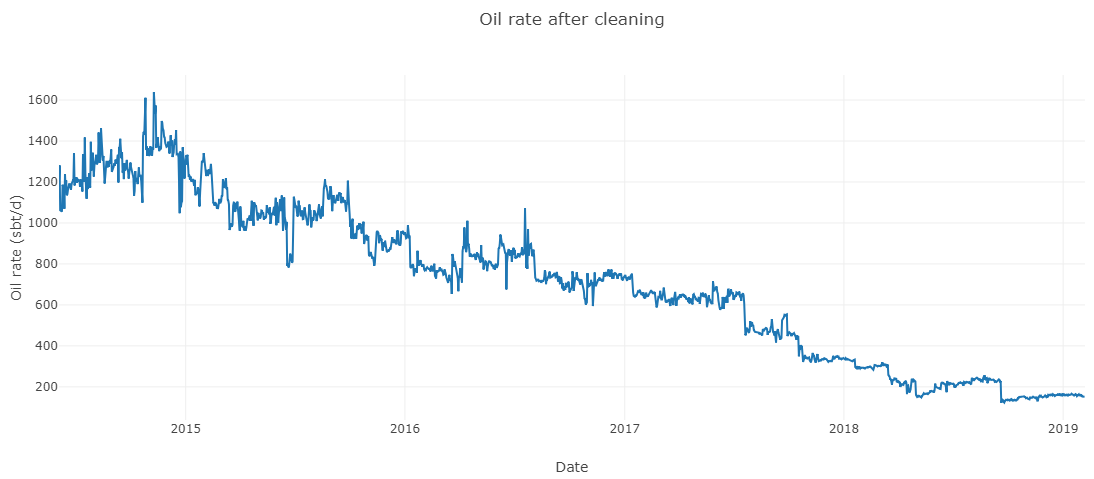
\includegraphics[scale=0.38]{fig/q_oil_after.PNG}
        \caption{Oil rate after remove outliers}
        \label{fig:q_oil_after}
    \end{figure}
\end{frame}
\begin{frame}{Data cleaning}
    \begin{figure}
        \centering
        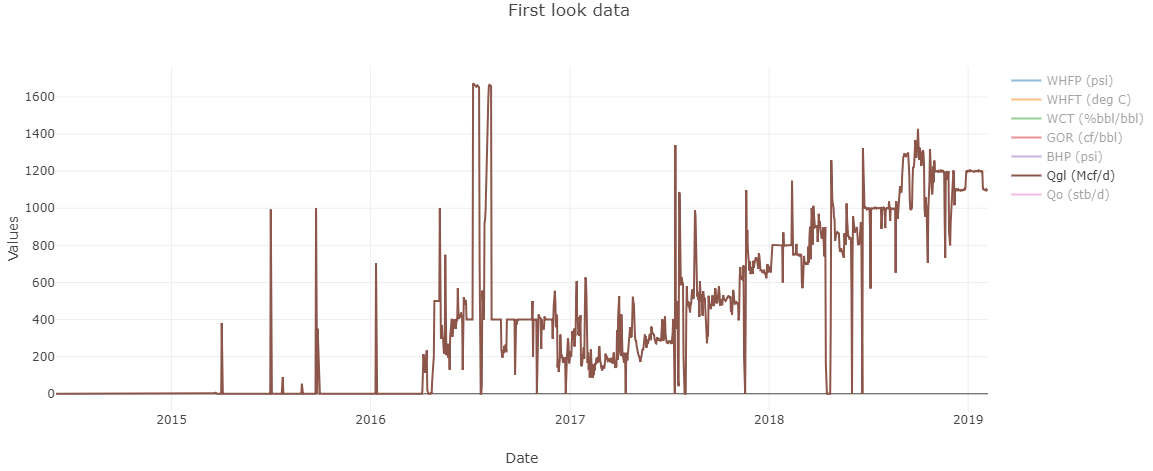
\includegraphics[scale=0.38]{fig/gl_before.PNG}
        \caption{Gaslift rate before remove outliers}
        \label{fig:gl_before}
    \end{figure}
\end{frame}
\begin{frame}{Data cleaning}
    \begin{figure}
        \centering
        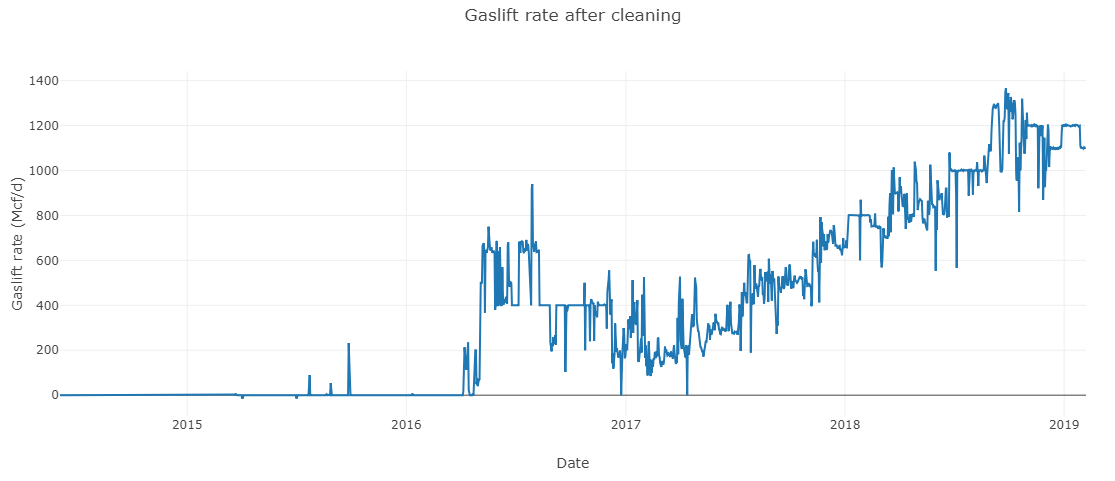
\includegraphics[scale=0.38]{fig/gl_after.PNG}
        \caption{Gaslift rate after remove outliers}
        \label{fig:gl_after}
    \end{figure}
\end{frame}
\begin{frame}{Data cleaning}
    \begin{figure}
        \centering
        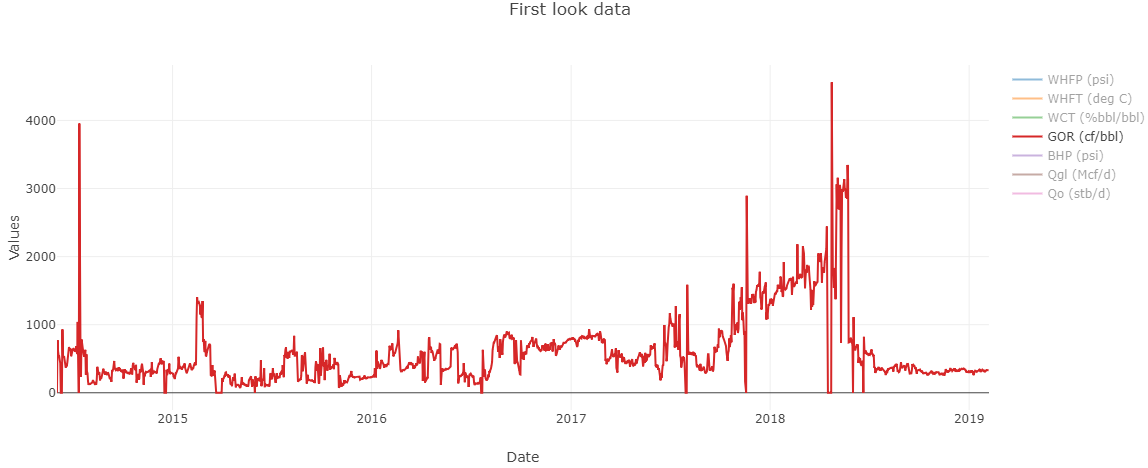
\includegraphics[scale=0.38]{fig/gor_before.PNG}
        \caption{Gas-oil ratio before remove outliers}
        \label{fig:gor_before}
    \end{figure}
\end{frame}
\begin{frame}{Data cleaning}
    \begin{figure}
        \centering
        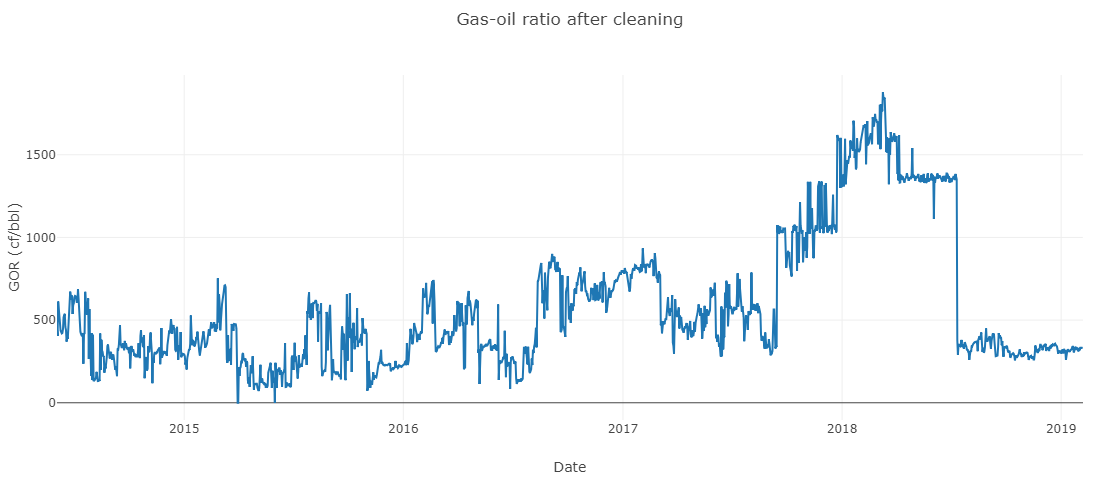
\includegraphics[scale=0.38]{fig/gor_after.PNG}
        \caption{Gas-oil ratio after remove outliers}
        \label{fig:gor_after}
    \end{figure}
\end{frame}
\begin{frame}{All features}
    \begin{figure}
        \centering
        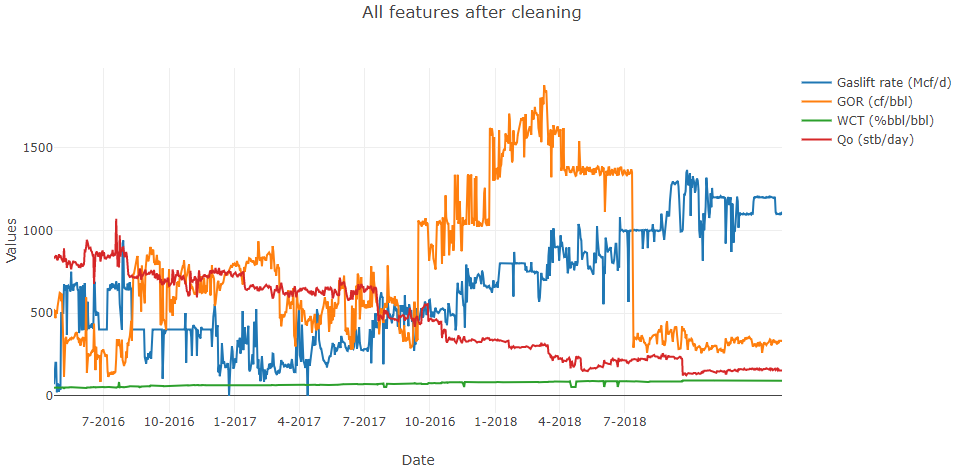
\includegraphics[scale=0.45]{fig/after.PNG}
        \caption{dataset after cleaning}
        \label{fig:after}
    \end{figure}
\end{frame}

\subsection{Data shifting}
\begin{frame}{Output shifting}
Make new feature with shifting backward output $n$ step, with $n = forcast times (days)$ (here n = 1).
    \begin{table}[h]
    \caption{First five row of new data}
    \begin{tabular}{@{}ccccc@{}}
    \toprule
    \textbf{\begin{tabular}[c]{@{}c@{}}Qgl\\ Mcf/d\end{tabular}} & \textbf{\begin{tabular}[c]{@{}c@{}}GOR\\ cf/bbl\end{tabular}} & \textbf{\begin{tabular}[c]{@{}c@{}}WCT\\ \%bbl/bbl\end{tabular}} & \textbf{\begin{tabular}[c]{@{}c@{}}new\\ STB/d\end{tabular}} & \textbf{\begin{tabular}[c]{@{}c@{}}Qo\\ STB/d\end{tabular}} \\ \midrule
    70.0                                                         & 525.0                                                         & 49.09                                                            & 843.59                                                       & 836.69                                                      \\
    150.0                                                        & 477.0                                                         & 49.77                                                            & 836.69                                                       & 842.81                                                      \\
    200.0                                                        & 469.0                                                         & 49.66                                                            & 842.81                                                       & 849.36                                                      \\
    200.0                                                        & 515.0                                                         & 48.87                                                            & 849.36                                                       & 827.09                                                      \\
    54.0                                                         & 495.0                                                         & 49.93                                                            & 827.09                                                       & 819.58                                                      \\ \bottomrule
    \end{tabular}
    \end{table}
    \begin{itemize}
        \item 1019 samples
        \item Date: from 4/23/2016
    \end{itemize}
\end{frame}
\section{Model architecture and Training}
\subsection{Model architecture}
\begin{frame}{Model architecture}
Model was configure with 5 nodes of input layer, 1 node of output layer without hidden layer.
\def\layersep{2.5cm}
\begin{tikzpicture}[shorten >=1pt,->,draw=black!50, node distance=\layersep]
    \tikzstyle{every pin edge}=[<-,shorten <=1pt]
    \tikzstyle{neuron}=[circle,fill=black!25,minimum size=17pt,inner sep=0pt]
    \tikzstyle{input neuron}=[neuron, fill=green!50];
    \tikzstyle{output neuron}=[neuron, fill=red!50];
    \tikzstyle{hidden neuron}=[neuron, fill=blue!50];
    \tikzstyle{annot} = [text width=4em, text centered]

    % Draw the input layer nodes
    \foreach \name / \y in {1,...,5}
    % This is the same as writing \foreach \name / \y in {1/1,2/2,3/3,4/4}
        \node[input neuron, pin=left:Input \#\y] (I-\name) at (1,-\y + 0.5) {};

    \node[output neuron,pin={[pin edge={->}]right:Output}, right of=I-3] (O) {};

    \foreach \source in {1,...,5}
        \path (I-\source) edge (O);

    % Annotate the layers
    \node[annot] at (1, 0.5) {Input Layer};
    \node[annot] at (3.5, 0.5) {Output Layer};
\end{tikzpicture}
\end{frame}

\subsection{Training}
\begin{frame}{Loss values}
``Loss" like error, in most cases, model has lower loss is more reliable.
    \begin{figure}
        \centering
        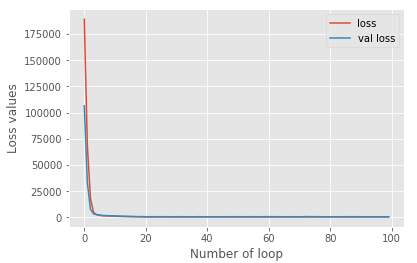
\includegraphics[scale=0.65]{fig/loss.png}
        \caption{Loss value with over 100 loops}
        \label{fig:loss}
    \end{figure}
\end{frame}

\section{Results and Evaluation}
\begin{frame}{Predict on test data}
    \begin{figure}
        \centering
        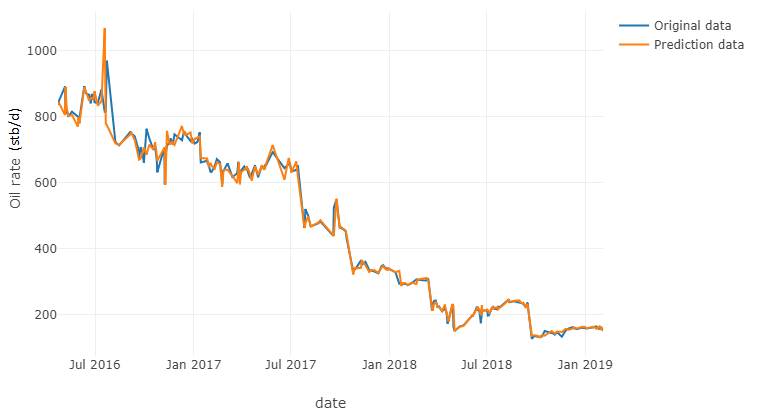
\includegraphics[scale=0.53]{fig/evalua.PNG}
        \caption{Predict results}
        \label{fig:evalua}
    \end{figure}
\end{frame}
\begin{frame}{Evaluation}
RMSE = 29.62, $R^2 = 98,55 \%$
    \begin{figure}
        \centering
        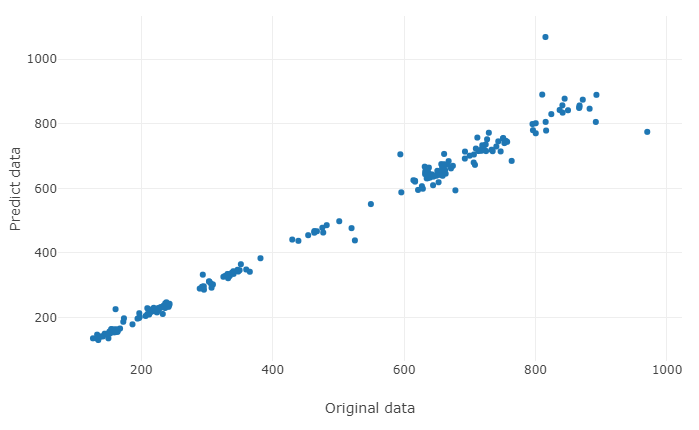
\includegraphics[scale=0.5]{fig/relationship.PNG}
        \caption{Evaluate predict data}
        \label{fig:relationship}
    \end{figure}
\end{frame}
\begin{frame}{Choose gas-lift rate}
Assume we have to choose gas-lift rate to obtain maximum oil rate in the next day (assume another features are defined):
\begin{table}[]
\begin{tabular}{cccccl}
\cline{1-5}
\textbf{\begin{tabular}[c]{@{}c@{}}Qgl\\ Mcf/d\end{tabular}} & \textbf{\begin{tabular}[c]{@{}c@{}}GOR\\ cf/bbl\end{tabular}} & \textbf{\begin{tabular}[c]{@{}c@{}}WCT\\ \%bbl/bbl\end{tabular}} & \textbf{\begin{tabular}[c]{@{}c@{}}new\\ STB/d\end{tabular}} & \textbf{\begin{tabular}[c]{@{}c@{}}Qo\\ STB/d\end{tabular}} &                              \\ \cline{1-5}
1000                                                         & 329                                                           & 90.5                                                            & 152                                                          & 154.1                                                       &                              \\
1102                                                         & 329                                                           & 90.5                                                            & 152                                                          & 153.8                                                       &                              \\
1110                                                         & 329                                                           & 90.5                                                            & 152                                                          & 152.2                                                       &                              \\ \hline
\multicolumn{1}{|c|}{\cellcolor[HTML]{CBCEFB}1096}           & \multicolumn{1}{c|}{\cellcolor[HTML]{CBCEFB}329}              & \multicolumn{1}{c|}{\cellcolor[HTML]{CBCEFB}90.5}               & \multicolumn{1}{c|}{\cellcolor[HTML]{CBCEFB}152}             & \multicolumn{1}{c|}{\cellcolor[HTML]{CBCEFB}154.5}          & \multicolumn{1}{l|}{Choosed} \\ \hline
1104                                                         & 329                                                           & 90.5                                                            & 152                                                          & 152.7                                                       &                              \\ \cline{1-5}
\multicolumn{1}{|l|}{}                                       & \multicolumn{2}{c|}{Assume are known}                                                                                           & \multicolumn{1}{c|}{Shifted}                                 & \multicolumn{1}{c|}{Predict}                                &                              \\ \cline{1-5}
\end{tabular}
\end{table}
\end{frame}
\section{Conclusion}
\begin{frame}{Conclusion}
- With this model, we can choose gaslift rate to obtain the maximum oil rate (in example we can choose 1096 (Mcf/d) to get 154.5 (stb.d))\\
- This study will be extend to optimize gas lift of multiple wells under constrain of total gaslift amount.\\
- This model rely on data, input data used to train need to be under preprocessed.\\
- More data more reliable.\\
- Evaluation and result in attach file.\\
- All source code here: \href{https://nbviewer.jupyter.org/github/YanGBloG/Data-Analysis/blob/a69fc2607dcad85ad33ff300e259fd8b1951c09b/Production\%20forcasting\%20with\%20MLP,\%20LSMT/predict-performance-mlp-gru.ipynb}{\textcolor{red}{\emph{[Click here]}}} 

\end{frame}
\subsection{Đề cương luận án}
\begin{frame}{Chương I: CỞ SỞ LÝ THUYẾT}
    \begin{itemize}
        \item[1.1.] Dự báo khai thác
            \begin{itemize}
                \item[1.1.1.] Các nguyên lý cơ bản
                \item[1.1.2.] Phân tích đường cong suy giảm
            \end{itemize}
        \item[1.2.] Các phương pháp khai thác nhân tạo
            \begin{itemize}
                \item[1.2.1.] Bơm điện chìm
                \item[1.2.2.] Gas lift
            \end{itemize}
    \end{itemize}
\end{frame}

\begin{frame}{Chương I: CỞ SỞ LÝ THUYẾT}
    \begin{itemize}
        \item[1.3.] Mạng neuron truyền thẳng
            \begin{itemize}
                \item[1.3.1.] Cấu trúc cơ bản
                \item[1.3.2.] Hàm kích hoạt
                \item[1.3.3.] Hàm tối ưu
                \item[1.3.4.] Phương pháp đánh giá
                    \begin{itemize}
                        \item[a)] Phương pháp bình phương tối thiểu
                        \item[b)] Phương pháp $R^2$
                    \end{itemize}
            \end{itemize}
        \item[1.4.] Giải thuật di truyền
            \begin{itemize}
                \item[1.4.1.] Nguyên lý cơ bản
                \item[1.5.1.] Thuật toán di truyền
            \end{itemize}
    \end{itemize}
\end{frame}

\begin{frame}{Chương II: TỔNG QUAN GIẾNG X1 MỎ RẠNG ĐÔNG}
    \begin{itemize}
        \item[2.1.] Mỏ Rạng Đông
        \item[2.2.] Giếng X1
    \end{itemize}
\end{frame}

\begin{frame}{Chương III: XÂY DỰNG, TRIỂN KHAI MÔ HÌNH}
    \begin{itemize}
        \item[A. ] Xây dựng mô hình dự báo lưu lượng khai thác dầu
    \end{itemize}
    \begin{itemize}
        \item[3.1.] Tiền xử lý dữ liệu
            \begin{itemize}
                \item[3.1.1.] Làm sạch dữ liệu
                    \begin{itemize}
                        \item[a)] Xử lí nhiễu, dữ liệu ngoại lai
                        \item[b)] Xử lí điểm mất dữ liệu
                    \end{itemize}
                \item[3.1.2.] Chuyển vị dữ liệu
            \end{itemize}
    \end{itemize}
\end{frame}

\begin{frame}{Chương III: XÂY DỰNG, TRIỂN KHAI MÔ HÌNH}
    \begin{itemize}
        \item[A. ] Xây dựng mô hình dự báo lưu lượng khai thác dầu
    \end{itemize}
    \begin{itemize}
        \item[3.2.] Xây dựng và huấn luyện mô hình
            \begin{itemize}
                \item[3.2.1.] Xây dựng cấu trúc
                \item[3.2.2.] Huấn luyện mô hình
                    \begin{itemize}
                        \item[a)] Huấn luyện
                        \item[b)] Kết quả
                    \end{itemize}
                \item[3.1.2.] Kết hợp mô hình
            \end{itemize}
    \end{itemize}
\end{frame}

\begin{frame}{Chương III: XÂY DỰNG, TRIỂN KHAI MÔ HÌNH}
    \begin{itemize}
        \item[B. ] Xây dựng mô hình giải thuật di truyền
    \end{itemize}
    \begin{itemize}
        \item[3.3.] Triển khai thuật toán
    \end{itemize}
    \begin{itemize}
        \item[C. ] Kết hợp mô hình giải thuật và mô hình dự báo cho giếng X1
    \end{itemize}
    \begin{itemize}
        \item[3.4.] Dự báo từng thành phần trong mô hình
        \item[3.5.] Lựa chọn lưu lượng gas lift với mô hình giải thuật di truyền
        \item[3.6.] Dự đoán lưu lượng dầu trong tương lai
    \end{itemize}
\end{frame}

\begin{frame}{KẾT LUẬN, KIẾN NGHỊ}
    \begin{itemize}
        \item[A. ] KẾT LUẬN
            \begin{itemize}
                \item Kết quả đạt được
            \end{itemize}
        \item[B. ] KIẾN NGHỊ
            \begin{itemize}
                \item Các kiến nghị
            \end{itemize}
    \end{itemize}
\end{frame}

\begin{frame}{}
    \begin{center}
    THANK YOU FOR ALL YOUR SUPPORTS
    \end{center}
\end{frame}

\end{document}